	%%%%%%%%%%%%%%%%%%%%%%%%%%%%%%%%%%%%%%%%%
	% baposter Landscape Poster
	% LaTeX Template
	% Version 1.0 (11/06/13)
	%
	% baposter Class Created by:
	% Brian Amberg (baposter@brian-amberg.de)
	%
	% This template has been downloaded from:
	% http://www.LaTeXTemplates.com
	%
	% License:
	% CC BY-NC-SA 3.0 (http://creativecommons.org/licenses/by-nc-sa/3.0/)
	%
	%%%%%%%%%%%%%%%%%%%%%%%%%%%%%%%%%%%%%%%%%

	%----------------------------------------------------------------------------------------
	%	PACKAGES AND OTHER DOCUMENT CONFIGURATIONS
	%----------------------------------------------------------------------------------------

	\documentclass[landscape,a0paper,fontscale=0.275]{baposter} % Adjust the font scale/size here, before (fontscale=0.285)

	\usepackage{graphicx} % Required for including images
	\graphicspath{{figures/}} % Directory in which figures are stored

	\usepackage{amsmath} % For typesetting math
	\usepackage{amssymb} % Adds new symbols to be used in math mode

	\usepackage{booktabs} % Top and bottom rules for tables
	\usepackage{enumitem} % Used to reduce itemize/enumerate spacing
	\usepackage{palatino} % Use the Palatino font
	\usepackage[font=small,labelfont=bf]{caption} % Required for specifying captions to tables and figures
	\usepackage{url} % To insert ~ in:http://d.umn.edu/~sivelab/

	\usepackage{multicol} % Required for multiple columns
	\setlength{\columnsep}{1.5em} % Slightly increase the space between columns
	\setlength{\columnseprule}{0mm} % No horizontal rule between columns

	% \usepackage{graphicx}% http://tex.stackexchange.com/questions/25887/how-to-move-a-whole-tikzpicture

	\usepackage{tikz} % Required for flow chart
	\usetikzlibrary{positioning,shapes,arrows} % Tikz libraries required for the flow chart in the template

	\newcommand{\compresslist}{ % Define a command to reduce spacing within itemize/enumerate environments, this is used right after \begin{itemize} or \begin{enumerate}
	\setlength{\itemsep}{1pt}
	\setlength{\parskip}{0pt}
	\setlength{\parsep}{0pt}
	}

	\definecolor{lightblue}{rgb}{0.145,0.6666,1} % Defines the color used for content box headers
	\definecolor{maroon}{rgb}{128,0,0} % Defines the color used for content box headers
	\begin{document}

	\begin{poster}
	{
	headerborder=closed, % Adds a border around the header of content boxes
	colspacing=1em, % Column spacing
	bgColorOne=white, % Background color for the gradient on the left side of the poster
	bgColorTwo=white, % Background color for the gradient on the right side of the poster
	% borderColor=lightblue, % Border color
	borderColor=maroon,
	headerColorOne=black, % Background color for the header in the content boxes (left side)
	% headerColorTwo=lightblue, % Background color for the header in the content boxes (right side)
	headerColorTwo=maroon,
	headerFontColor=white, % Text color for the header text in the content boxes
	boxColorOne=white, % Background color of the content boxes
	textborder=roundedleft, % Format of the border around content boxes, can be: none, bars, coils, triangles, rectangle, rounded, roundedsmall, roundedright or faded
	eyecatcher=true, % Set to false for ignoring the left logo in the title and move the title left
	headerheight=0.1\textheight, % Height of the header
	headershape=roundedright, % Specify the rounded corner in the content box headers, can be: rectangle, small-rounded, roundedright, roundedleft or rounded
	headerfont=\Large\bf\textsc, % Large, bold and sans serif font in the headers of content boxes
	%textfont={\setlength{\parindent}{1.5em}}, % Uncomment for paragraph indentation
	linewidth=2pt % Width of the border lines around content boxes
	}
	%----------------------------------------------------------------------------------------
	%	TITLE SECTION
	%----------------------------------------------------------------------------------------
	%
	% {
\includegraphics[height=4em]{logo.png}} % First university/lab logo on the left
	{
\includegraphics[height=4em]{UMD.png}}
	{\bf\textsc{Human Steerable Genetic Alogrithm Application}\vspace{0.5em}} % Poster title
	{\textsc{\{ Penghuan Ni, Rich Maclin and Peter Willemsen \} \hspace{12pt} University of Minnesota Duluth}} % Author names and institution
	% {
\includegraphics[height=4em]{logo.png}} % Second university/lab logo on the right
	{
\includegraphics[height=4em]{UMN.jpg}}

	%----------------------------------------------------------------------------------------
	%	REFERENCES
	%----------------------------------------------------------------------------------------

	\headerbox{References}{name=references,column=0,above=bottom}{

	\renewcommand{\section}[2]{\vskip 0.05em} % Get rid of the default "References" section title
	\nocite{*} % Insert publications even if they are not cited in the poster
	\small{ % Reduce the font size in this block
	\bibliographystyle{unsrt}
	\bibliography{sample} % Use sample.bib as the bibliography file
	}}

	%----------------------------------------------------------------------------------------
	%	INTRODUCTION
	%----------------------------------------------------------------------------------------

	\headerbox{Introduction}{name=introduction,column=0,row=0,above=references}{

	Genetic Algorithm(GA) which imitates the process of natural selection has been applied into Artificial Intelligence area for a long time. From when GA was introduced to now, GA has been discussed and developed so many times. For some specific problems, we want to make some changes for GA. In our research, we will develop a human steerable genetic algorithm and apply it on the Optimization of Urban Design problem.

	To find the optimal solution for the Urban Design problem, we will take dynamic factors into account, such as:
	\begin{enumerate}\compresslist
	\item the location and height of a building
	\item wind energy and solar energy
	\item use wind to blow the air pollution
	\end{enumerate}

	Also, the human steerable GA could consider people's opinions. It will ask feedback from the users, which could change the direction of GA reproduction process.\\

	By using the human steerable genetic algorithm, we expect to have a human preferred solution for urban design problem. Human can select different method for selection, crossover, and mutation operations. When we run the human interacted GA, people can change the fitness value for some of the chromosome based on their preference. \\

	Our method will be a good reference for the future cities designers. Designers could use it to make a cleaner, more eco-friendly, and more comfortable city. Moreover, citizens could also participate in the city design, by giving feedback to the GA system.
	% \begin{enumerate}\compresslist
	% \item
	% \item
	% \end{enumerate}

	\vspace{0.3em} % When there are two boxes, some whitespace may need to be added if the one on the right has more content
	}

	%----------------------------------------------------------------------------------------
	%	GA EXPLAINATION
	%----------------------------------------------------------------------------------------

	\headerbox{GA Explanation}{name=gaexplanation,column=1,span=2,row=0}{

	\begin{multicols}{2}

	% Define block styles

	\tikzstyle{decision} = [diamond, draw, fill=blue!20,
	text width=4.5em, text badly centered, node distance=2.5cm, inner sep=0pt]
	\tikzstyle{block} = [rectangle, draw, fill=blue!20, node distance=2cm,
	text width=6em, text centered, rounded corners, minimum height=1em]
	\tikzstyle{line} = [draw, -latex']
	\tikzstyle{cloud} = [draw, ellipse,fill=red!20, node distance=3cm,
	minimum height=2em]

	\hspace*{1.5em}\vspace*{1.5em}{
		\begin{tikzpicture}[node distance = 2cm, auto]
		% \hspace*{3em}
		% Place nodes
		\node [block] (init) {start};
		\node [block, text width=10em, below = .8cm of init] (initpop) {generate initial population};
		\node [block, below = .81cm of initpop] (calcfitness) {calculate fitness of each individual };
		%     \node [block, below of=initpop] (evaluate) {evaluate candidate models};
		%     \node [block, left of=evaluate, node distance=3cm] (update) {update model};
		\node [block, below = .8cm of calcfitness] (newpop) {create new population};
		\node [block, right = 1.5cm of newpop] (crossover) {crossover};
		\node [block, above = 1cm of crossover] (selection) {selection};
		\node [block, below = 1cm of crossover] (mutation) {mutation};
		\node [block, below = 1cm of mutation, fill=red!20] (feedback) {feedback};
		\node [decision, below = .8cm of newpop] (decide) {end condition};

		\node [block, below = .8cm of decide, node distance=2cm] (stop) {stop};
		    % Draw edges
	    \path [line] (init) -- (initpop);
	    \path [line] (initpop) -- (calcfitness);
	    \path [line] (calcfitness) -- (newpop);
	    \path [line] ([yshift=0.1cm] newpop.east) -| ([xshift=-.82cm] selection.west) -- (selection.west);
	    \path [line] (selection) -- (crossover);
	    \path [line] (crossover) -- (mutation);
	    \path [line, dashed, draw=red!80] (mutation) -- (feedback);
	    \path [line, dashed, draw=red!80] (feedback) -| ([xshift=-0.8cm] mutation.west);
	    \path [line] (mutation) -| ([xshift=.7cm, yshift=-0.1cm] newpop.east) -- ([yshift=-0.1cm] newpop.east);
	    \path [line] (newpop) -- (decide);
	    \path [line] (decide) -| node [near start] {no} ([xshift=-1.5cm] newpop.west) -- (newpop);
		\path [line] (decide) -- node {yes}(stop);
		\end{tikzpicture}
	}

	\vspace{3em}

	\begin{itemize}\compresslist
	\item User specified parameters: number of variables, possible value of each variable, size of population, number of generations, fitness function, crossover probability, mutation probability, selection type, crossover type, and mutation type.
	\item Generate new population: generate the first generation of the solutions.
	\item Create new population: applying selection, crossover, and mutation to the previous generation, and get a new population, which should improve the solution.
	% \item Encoding method: binary encoding, use binary string to represent each variable
	\item Selection: selection a pair of parents and do the crossover and mutation operation on them. Support method is roulette-wheel.
	\item Crossover: exchange bits of binary string between two parents based on crossover probability and produce two children. Support methods are single-point, two-point and uniform.
	\item Mutation: mutate bits of children's binary strings based on mutation probability. Support methods is flip-bits.
	\end{itemize}

	\end{multicols}
	}

	%----------------------------------------------------------------------------------------
	%	STEERABLE GA
	%----------------------------------------------------------------------------------------

	\headerbox{Steerable GA}{name=steerablega,column=3,row=0,bottomaligned=gaexplanation}{

	% \tikzstyle{decision} = [diamond, draw, fill=blue!20,
	% text width=4.5em, text badly centered, node distance=2.5cm, inner sep=0pt]
	% \tikzstyle{block} = [rectangle, draw, fill=blue!20, node distance=2cm,
	% text width=6em, text centered, rounded corners, minimum height=1em]
	% \tikzstyle{line} = [draw, -latex']
	% \tikzstyle{cloud} = [draw, ellipse, fill=red!20, node distance=3cm,
	% minimum height=2em]

	% \hspace*{2.0em}{
		% \begin{tikzpicture}[node distance = 2cm, auto]
		% % \hspace*{3em}
		% % Place nodes
		% \node [block, text centered, minimum height=12em] (ga) {Genetic Algorithm};
		% \node [block, right = 1.5cm of ga, yshift=1.7cm, fill=red!20] (feedback1) {feedback1};
		% \node [block, below = .5cm of feedback1, fill=red!20] (feedback2) {feedback2};
		% \node [block, below = .5cm of feedback2, fill=red!20] (feedback3) {feedback3};
		% \node (e1)[below = 0.4 cm of feedback3]{\LARGE .};
		% \node (e2)[below = 0.6 cm of feedback3]{\LARGE .};
		% \node (e3)[below = 0.8 cm of feedback3]{\LARGE .};
		% \node [block, below = 1.2cm of feedback3, fill=red!20] (feedbackN) {feedbackN};

		%     % Draw edges
	 %    \path [line] (feedback1.west) -- (feedback1.west -| ga.east);
	 %    \path [line] (feedback2.west) -- (feedback2.west -| ga.east);
	 %    \path [line] (feedback3.west) -- (feedback3.west -| ga.east);
	 %    \path [line] (feedbackN.west) -- (feedbackN.west -| ga.east);

		% \end{tikzpicture}
	% }
	% \begin{figure}
	%   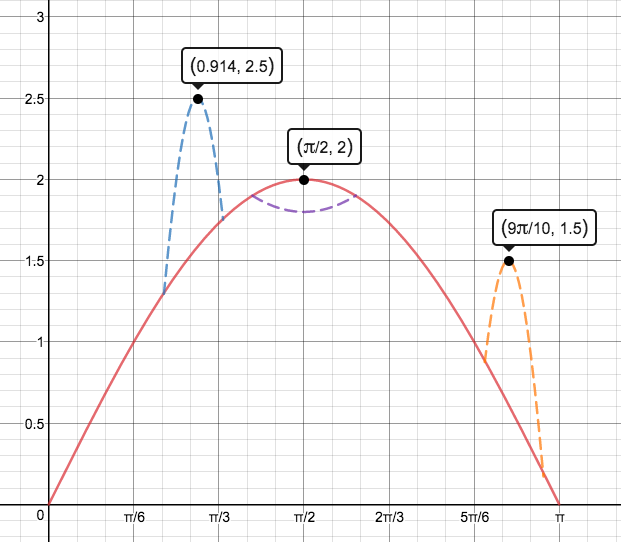
\includegraphics[width=\linewidth]{2sin.png}
	%   \caption{A boat.}
	%   \label{fig:boat1}
	% \end{figure}

	{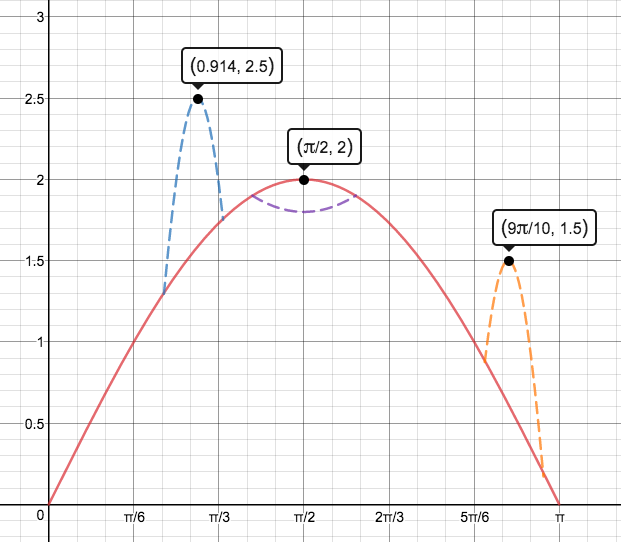
\includegraphics[height=18em]{2sin.png}}

	For example, we have a one variable equation which is 2*sin(x), in domain between 0 and pi, and we want to find the maximum value of it. Obviously, when x equals pi/2 we get the optimal solution. However, for some reason, we can not select from that region, instead, we think when x equals 0.914 or 9*pi/10, we can have better result. So we increase the probability to get those two values as our result by giving the GA our feedback such as, like or dislike.

	% \begin{itemize}\compresslist
	% \item GA is running at server side.
	% \item Different users give feedback to GA. In our case, those feedback could be the suggestion of the height or location of a building, if the user like a particular solution or not, etc.
	% \item GA takes users feedbacks into account and reproduces the solutions.
	% \item While users keep giving the GA feedback, GA could generate user preferred solutions.
	% \item When the solution converge at some solutions, the GA will terminate itself.
	% \end{itemize}


	}

	%----------------------------------------------------------------------------------------
	%	FUTURE RESEARCH
	%----------------------------------------------------------------------------------------

	\headerbox{Future Research}{name=futureresearch,column=1,span=2,aligned=references,above=bottom}{ % This block is as tall as the references block

	\begin{multicols}{2}
	Our GA has all the genetic algorithm functionalities, however, different variants should be use for different problems. Everyone is welcome to pull our code from Github and make changes for their uses.

	We applied our human steerable GA in Urban Design Optimization problem, in the future, people could apply it on other complex problems, which human's opinions should take into account.

	\end{multicols}
	}

	%----------------------------------------------------------------------------------------
	%	CONTACT INFORMATION
	%----------------------------------------------------------------------------------------

	\headerbox{Contact Information}{name=contact,column=3,aligned=references,above=bottom}{ % This block is as tall as the references block

		\begin{description}
		% \begin{itemize}
		\compresslist
			\item[Web] \url{www.d.umn.edu/~sivelab/}
			\item[Email] nixxx136@d.umn.edu
			\item[Address] University of Minnesota Duluth, Computer Science Department
		% \end{itemize}
		\end{description}
	}

	%----------------------------------------------------------------------------------------
	%	CURRENT RESULTS
	%----------------------------------------------------------------------------------------

	\headerbox{Current Results}{name=results,column=1,span=3,row=1,below=gaexplanation,above=references}{

	\begin{multicols}{3}
	On the right side, we have two simple configuration for two by two blocks. In the configuration:

	\begin{enumerate}\compresslist
	\item B means Building area
	\item G means Park area
	\item P means Parking area
	\end{enumerate}

	Our algorithm will give us the best solution for this toy example.

	\vfill
	\columnbreak

	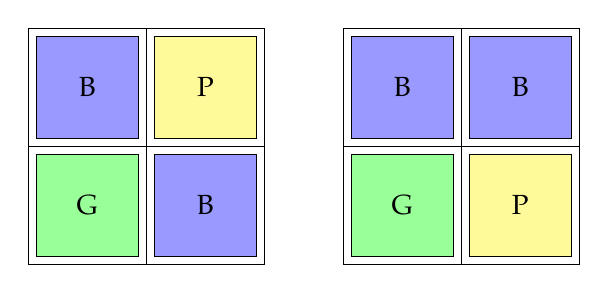
\begin{tikzpicture}

	\draw[black, thin] (0,0) -- (3,0) -- (3,-3) -- (0,-3) -- (0,0);
	\draw[black, thin] (0,-1.5) -- (3,-1.5);
	\draw[black, thin] (1.5,0) -- (1.5,-3);

	\filldraw[fill=blue!40!white, draw=black, thin] (0.1,-0.1) rectangle (1.4,-1.4) node[pos=.5] {B};
	\filldraw[fill=green!40!white, draw=black, thin] (0.1,-1.6) rectangle (1.4,-2.9) node[pos=.5] {G};;
	\filldraw[fill=blue!40!white, draw=black, thin] (1.6,-1.6) rectangle (2.9,-2.9) node[pos=.5] {B};;
	\filldraw[fill=yellow!40!white, draw=black, thin] (1.6,-0.1) rectangle (2.9,-1.4) node[pos=.5] {P};;

	\draw[black, thin] (4,0) -- (7,0) -- (7,-3) -- (4,-3) -- (4,0);
	\draw[black, thin] (4,-1.5) -- (7,-1.5);
	\draw[black, thin] (5.5,0) -- (5.5,-3);

	\filldraw[fill=blue!40!white, draw=black, thin] (4.1,-0.1) rectangle (5.4,-1.4) node[pos=.5] {B};
	\filldraw[fill=green!40!white, draw=black, thin] (4.1,-1.6) rectangle (5.4,-2.9) node[pos=.5] {G};;
	\filldraw[fill=yellow!40!white, draw=black, thin] (5.6,-1.6) rectangle (6.9,-2.9) node[pos=.5] {P};;
	\filldraw[fill=blue!40!white, draw=black, thin] (5.6,-0.1) rectangle (6.9,-1.4) node[pos=.5] {B};;

	\end{tikzpicture}

	\columnbreak

	When we run the program, we have a environment simulation function, which could help us to evaluate each configuration to get a fitness value. Moreover, people could also select which configuration they like or dislike to affect the fitness value. Since this is only a 2*2 blocks, the number of blocks and combinations are small, but when we have a 200*200 blocks, we will see the advantage of our algorithm.

	\end{multicols}
	% 	\vspace{-2em}
	}

	%----------------------------------------------------------------------------------------

	\end{poster}

	\end{document}
